\section{Architecture}

WHAT is based upon a intransparend multitier architecture. 
The GUI, presentation logic, application processing, data accessing and stroring data
are logically and also partly locally separated. Intransparend means that communication
between tiers just happens between adjacent ones. The different tiers are described below.


\begin{center}
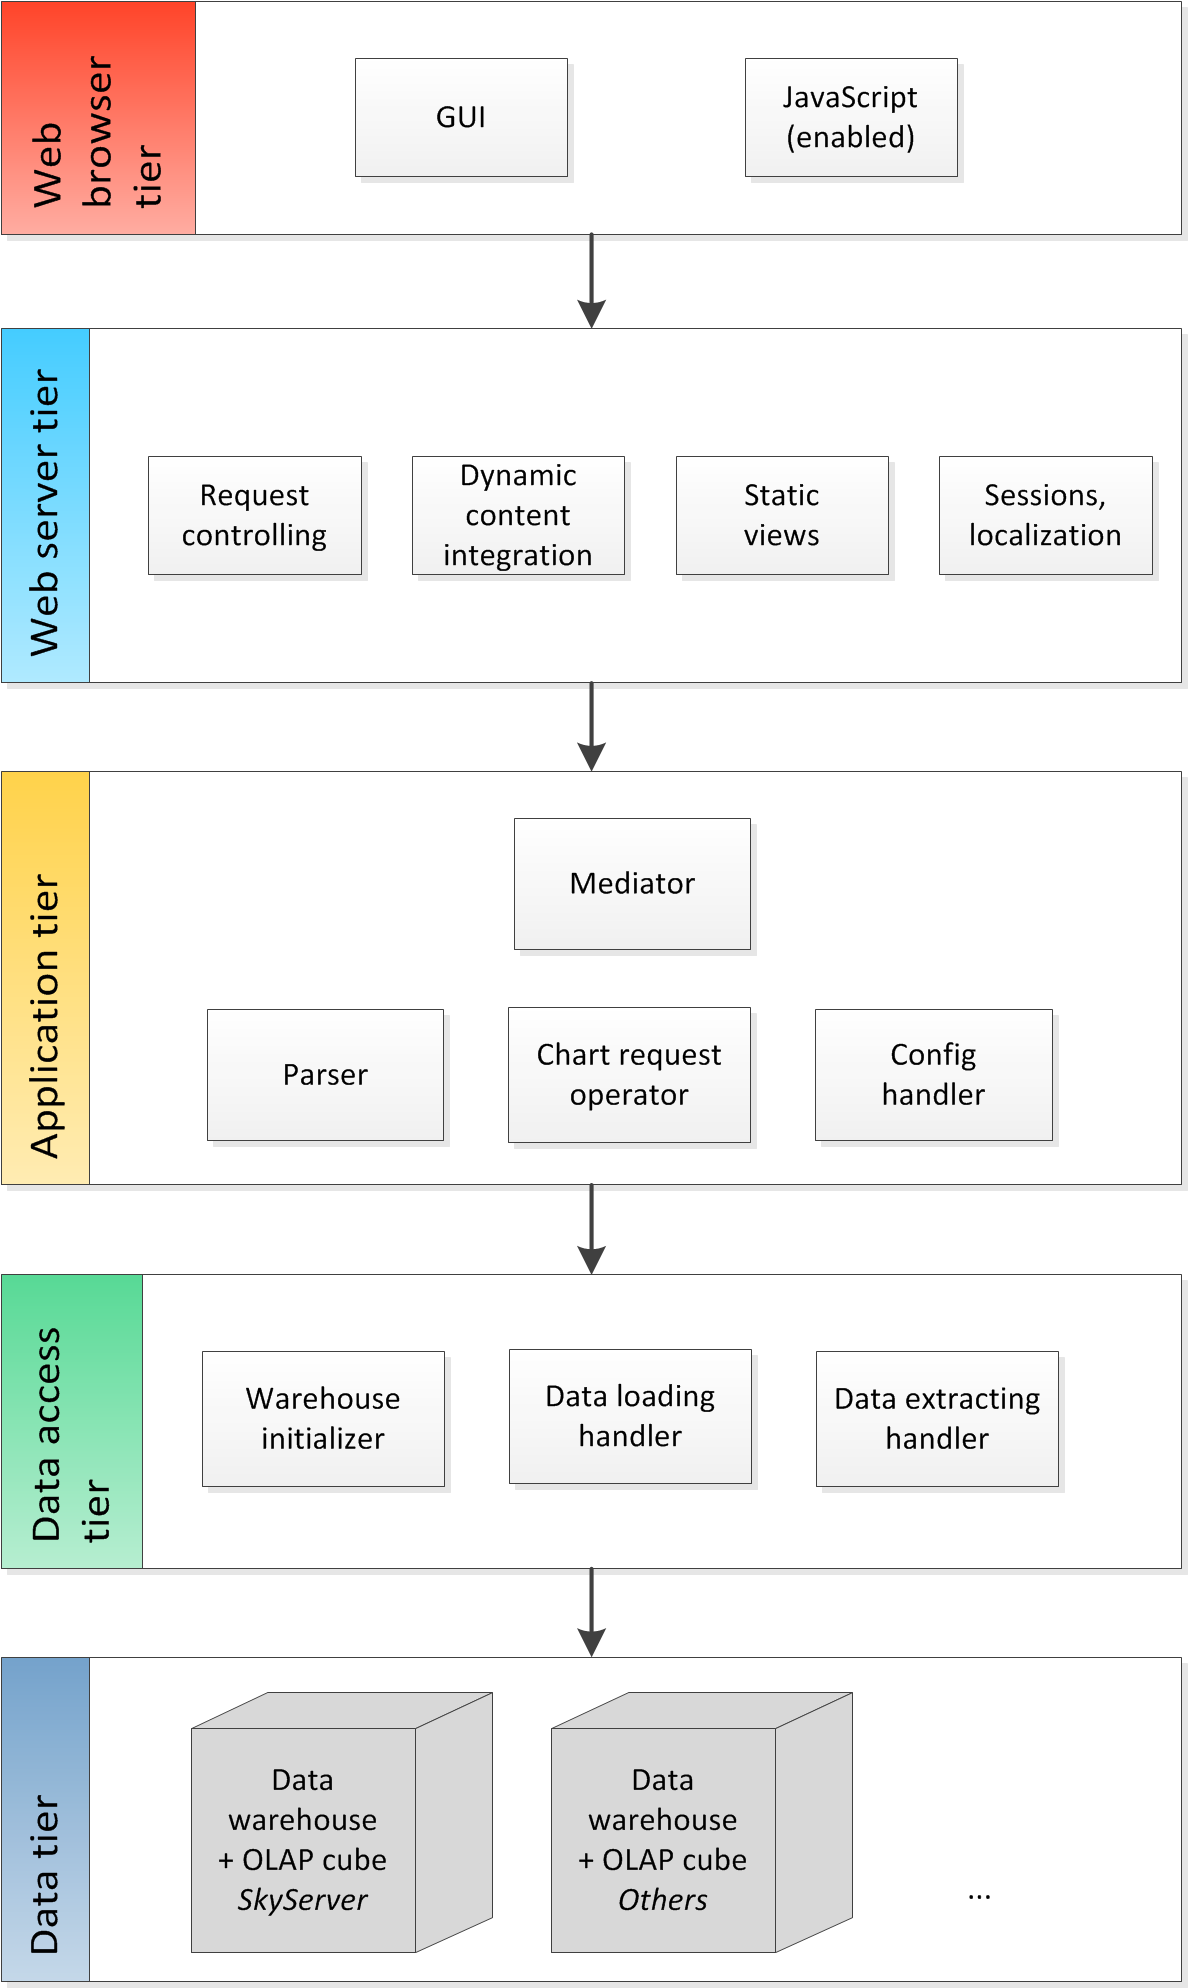
\includegraphics[width=0.6\linewidth]{Pictures/TierArchi.png} 
\end{center}   


\subsection{Web browser tier}
The web browser tier represents the web browser of the client on which the GUI, a web page, will be displayed.
As the web page uses JavaScript, this has to be enabled in the browser. 
Besides this, Google Chrome and Firefox have to be supported. 


\subsection{Web server tier}
The web server provides the presentation logic. This includes static html-pages and integration of dynamic
conent. Other tasks are sessioning, localization (languages) and most important request controlling. 
Which means it handles the actions triggered on the web page and decides whether it can handle them itself 
or pass them to application tier. Last one happens for example when a chart is requested. 
The Java Play framework is used in this tier.


\subsection{Application tier}
In the application tier the parsing process, managing the configuration files and above all 
the chart computing are taking place. 

\subsection{Data access tier}
This tier manages all requests of loading and extracting data from the data tier. So his main task is
to build a bridge from the application in Java to the SQL language of the Oracle warehouses and OLAP-Cubes.
If there is enough time to implement this optional function, it will also handle 
the automatic initialization of new data warehouses.  

\subsection{Data tier}
In the data tier the data warehouses and their OLAP-Cubes are stored. 
This will be done with the Oracle software.  
